\chapter{Soporte Fisico}

Al igual que en los capítulos anteriores, mostraremos cuál ha sido el desarrollo realizado para llevar, en este caso, el robot GopiGo3 a la plataforma Kibotics, lo que permitirá su programación.

\section{Características del Robot GoPiGo3}

GoPiGo es un robot fabricado por Dexter Industries \footnote{\url{https://www.dexterindustries.com}}, que pretende integrar la Raspberry Pi en los robots, dotándoles así de una mayor capacidad y flexibilidad. Actualmente se encuentra en su versión GoPiGo3, que consiste en un kit robótico con forma de vehículo (Figura 6.1).
\\
\begin{figure}[h!]
  \centering
    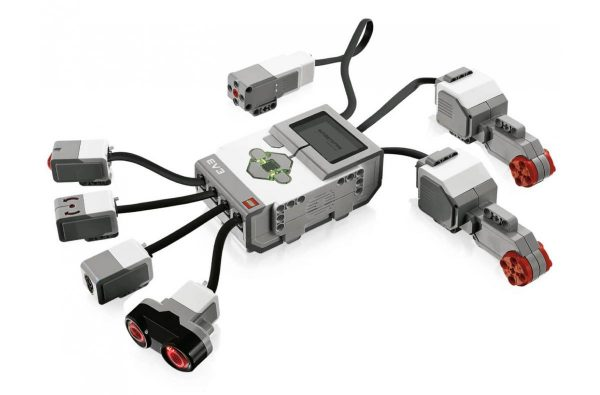
\includegraphics[width=0.8\textwidth]{img/motoresysensores.jpg}
  \caption{Diseño hardware del Ev3}
  \label{Diseño hardware del Ev3}
\end{figure}
\\
Entre las características del \textit{hardware} del GoPiGo3 destaca su cuerpo, que consiste en un acrílico grueso. Requiere un voltaje de entre 7-12V, conseguible con una batería a pilas. Dispone de una placa llamada “GoPiGo3", que se conecta a la Raspberry Pi. La comunicación con la controladora se produce a través de la interfaz SPI (\textit{Serial Peripheral Interface}). Incluye dos motores para conectarlo a las ruedas, las cuales tienen 66,5 mm de diámetro. También dispone de codificadores electrónicos, que se conectan a los motores para mejorar la movilidad. Respecto a las interfaces externas, destacan los dos puertos I2C (\textit{Inter-Integrated Circuit}) y los puertos serie que están acoplados a los pines de la Raspberry Pi (Dexter Industries, 2020).
\\
\\
Dexter Industries también ha desarrollado DexterOS, que incluye el \textit{software} necesario para que la Raspberry Pi funcione con GoPiGo3 (Dexter Industries, 2020). DexterOS se distribuye mediante una SD (\textit{Secure Digital}) de 8GB que se inserta en la ranura de la Raspberry Pi. Este \textit{software} emite una señal \textit{WiFi} que, una vez que el usuario se ha conectado a ese punto de acceso, al acceder al navegador se obtiene una web que permite interactuar con el robot sin necesidad de realizar ninguna descarga previa en el ordenador (Figura 6.2).
\\
\begin{figure}[h!]
  \centering
    
\includegraphics[width=0.6\textwidth]{img/logo_vect.png}
  \caption{Sotfware para GoPiGo3}
  \label{Sotfware para GoPiGo3}
\end{figure}
\\
Esta web dispone de cuatro módulos. El primero incluye lecciones integradas para aprender a programar el GoPiGo3 y algunos conceptos sobre los sensores de los que dispone. Otro módulo ofrece la posibilidad de conducir el GoPiGo3 de forma remota. Los otros dos módulos sirven como editores para programar el robot, de manera que uno de ellos permite programarlo mediante un lenguaje basado en bloques llamado \texttt{Bloxter} (Figura 6.3), muy similar a \texttt{Blockly} y diseñado por la propia empresa, mientras que el otro sirve para programarlo en \texttt{Python} (Dexter Industries, 2020). También han creado librerías que facilitan su programación para este lenguaje (una de ellas se llama \texttt{EasyGoPiGo3}).
\\


\section{Diseño}

La figura 6.4 muestra el diseño seguido para integrar el GoPiGo3 real a la plataforma Kibotics. En comparación con el diseño para los dos robots anteriores, en este caso se utiliza un servidor adicional \texttt{Flask} que permitirá la recepción del programa en el robot en su procesador Raspberry Pi.
\\
\begin{figure}[h!]
  \centering
    \includegraphics[width=0.8\textwidth]{img/esquema.JPG}
  \caption{Diseño para la integración del GoPiGo3. La línea roja indica los componentes que deben estar conectados a la misma red WiFi}
  \label{Diseño para la integración del GoPiGo3}
\end{figure}
\\
El proceso consta de 5 pasos y en las siguientes secciones se profundizará en cada una de las partes y en las interacciones necesarias entre el cliente, el servidor de Kibotics y el servidor \texttt{Flask} de la Raspberry Pi, que permitirá programar al GoPiGo3 desde el navegador web usando Kibotics.

\section{Lado Cliente}

En la parrilla de unidades de Kibotics, se pueden encontrar varios ejercicios dedicados al GoPiGo3 para \texttt{Python}. Actualmente solo está disponible para este lenguaje.
\\
\\
En una de secciones del ejercicio se proporciona información al usuario sobre cómo realizar el envío, así como de las instalaciones que deben realizar. En este caso solo tiene que hacer instalaciones en la Raspberry Pi del robot, ya que en el ordenador del anfitrión no es necesaria ninguna instalación. En el fragmento 6.1 se muestran los detalles de cómo se ha diseñado esta sección.
\\
\begin{lstlisting}[frame=single,breaklines=true, label=Página de información del GoPiGo3, caption=Página de información del GoPiGo3,  captionpos=b]
<html>
<head>
<meta charset='UTF-8'><meta name='viewport' content='width=device-width initial-scale=1'>
<title>GoPiGo3</title></head>
<body><h1>GoPiGo3 example</h1>
<p>Podras realizar tu programa para enviarselo al GoPiGo.</p>
<p><img src="" width=200px></p>

<h2>1 - Instalacion</h2>
<ul>
 <li type="circle">
  <h4>   <b>En la Raspberry Pi 3 del GoPiGo3:</b> </h4>
   <ol start='1' >
    <li>
     Descargar el siguiente fichero comprimido => <a href="" target="_blank">Intalador</a>
    </li>
    <li>
     Descomprimir el Zip descargado y situarlo en el directorio /home/pi/
    </li>
    <li>
     Ir al directorio e instalar los drivers necesario, para ello abrir un terminal y ejecutar
    </li>
    <ol start='1' >
     <li>
      <code>chmod +x instalar_drivers_GoPiGo.sh</code>
     </li>
     <li>
      <code>./instalar_drivers_GoPiGo.sh</code>
     </li>
    </ol>
    <li>
     Agregar la instruccion que permite levantar siempre el servidor al encenderse la Raspberry, para ello dirigirse al directorio y abrir un terminal:</li> 
     <ol start='1' >
      <li>
       Ejecutar => <code>chmod +x iniciar_servidor_GoPiGo.sh</code>
      </li> 
      <li>
       Abrir el servicio cron => <code>crontabl -e</code>
      </li> 
      <li>
       Agregar la tarea <code> @reboot /home/pi/configuracion_GoPiGo/iniciar_servidor_GoPiGo.sh &</code>
      </li> 
     </ol>
   </ol>
   </li>
   <li type="circle">
    <h4>   <b>En el ordenador MacOS/Linux/Windows:</b> </h4>
     <p>No es necesaria ningun tipo de instalacion adicional para el funcionamiento.</p>
    </li>
</ul>

<h2>2 - Ejecucion</h2>
<ol start='' >
 <li>
  Realice su programa
 </li>
  <li>
   Eciende el GoPiGo y asegurate de que esta conectado a el WiFi. 
  </li>
  <li>
   Pulse en <b>Enviar</b>, si todo ha ido bien se cargara el programa en el GoPiGo3. 
  </li>
</ol>
</body>
</html>
\end{lstlisting}

\subsection{Editor en el navegador web}

Para escribir un programa y enviarlo al robot desde el lado del cliente, otra sección de la página web del ejercicio proporciona un editor donde el usuario podrá escribir su programa utilizando el lenguaje \texttt{Python}. En el editor se importa la librería “\texttt{EasyGoPigo3}” (Dexter Industries, 2018), que proporciona una API para interactuar con los sensores y actuadores del robot 

\subsection{Envío del código al servidor Flask en el robot}

Una vez que el usuario ha escrito el programa deseado, deberá pulsar el botón “Enviar” que puede verse en la figura 6.5, el cual desencadenará todo el proceso de envío. En el fragmento 6.2 se muestra cuál es el código HTML que permite iniciar este proceso.
\\
\begin{lstlisting}[frame=single,breaklines=true, label=Sección para el envío, caption=Sección para el envío,  captionpos=b]
<center><h3>En esta seccion podras enviar tu codigo  al GoPiGo3.</h3></center>

<div class="text-center">
 <img class="text-center" src="{{ exercise.language }}/{{ exercise.exercise_id }}/img/GoPiGo3.png" width="300px" height="250px">
</div>

<div id="text" class="text-center">
 <h3><span id="proxy_state" class="label label-success">Conexion con proxy</span></h3>
  <button type="button" id="send_mbot" class="btn btn-info" onclick="send_code_to_GoPiGo()">
   <span class="glyphicon glyphicon-send"></span> Enviar
  </button>
</div>
\end{lstlisting}
Tras pulsar el botón de envío, desde el navegador se manda al servidor \texttt{Flask} levantado en la Raspberry Pi del robot, el código del programa que se había escrito previamente en el editor. Este código se envía como un \textit{query parameter} de una petición GET haciendo uso de la función \texttt{fecth()}, de forma similar que en los capítulos anteriores.
\\
\begin{lstlisting}[frame=single,breaklines=true, label=Función de envío del código al servidor del GopiGo3, caption=Función de envío del código al servidor del GopiGo3,  captionpos=b]
function send_code_to_GoPiGo() {
   var editor = ace.edit("ace");
   let code = editor.getValue();
   console.log(code);
   const message = {
      method: "GET"
   };
   url = 'http://192.168.1.200:8001/run?python_code=' + JSON.stringify(code);
   fetch(url, message)
      .then(function(response) {
         if(response.ok){
            responseOk = true
         }else{
            responseOk = false
         }
           return response.text();
         })
      .then(function(data) {
         if(responseOk){
            console.log("Ok")
         }else{
            console.log("Send Fail")
         }

      })
      .catch(function(err) {
         console.error(err);
      });
}
\end{lstlisting}
El servidor \texttt{Flask} recibirá el código y realizará una serie de acciones (sección 6.5) que permitirán cargar el programa al robot.

\section{Lado Servidor Kibotics}

Este servidor no toma un papel tan importante para el proceso de envío del programa al GoPiGo3 como sí lo tenía para el Mbot y el dron Tello. En ellos, además de servir las páginas necesarias al navegador que permiten ir al ejercicio concreto del robot, a la sección de información o al editor, era el encargado de manipular el código fuente, de crear el ejecutable o de realizar el empaquetado que se enviaba al robot.
\\
\\
En este diseño, una vez que el código está escrito en el editor web, es enviado al servidor de kibotics para el guardado del ejercicio del usuario y al servidor \texttt{Flask} del robot para procesarlo y ejecutarlo. 

\section{Lado GoPiGo3}

La Raspberry Pi del GoPiGo3 toma un papel muy importante en el proceso de envío del programa al robot, puesto que en ella se tendrá montado un servidor \texttt{Flask} HTTP, que recibirá las peticiones del cliente y contendrá la lógica para la ejecución del programa recibido.
\\
\\
A diferencia del ordenador anfitrión, donde no se requería ninguna instalación para el envío del programa, en la Raspberry Pi sí hay que realizar unas instalaciones previas para poder utilizarse en el GopiGo3.

\subsection{Preparación del ordenador a bordo del GoPiGo3}

La preparación de la Raspberry Pi requiere una serie de procesos.

\begin{enumerate}
	\item \textit{Instalar sistema operativo}
	\\
	\\
	La Raspberry Pi necesita un sistema operativo. Aunque existen varios que puede soportar, se debe utilizar \texttt{Raspbian}, un sistema operativo optimizado para ella y basado en Debian, una distribución GNU/Linux.
	\item \textit{Instalación de los drivers y configuración} 
	\\
	\\
	Se deben instalar los \textit{drivers} y las librerías necesarias para que pueda interactuar con los sensores y actuadores del robot GoPiGo3. También es indispensable que esté conectada a la misma red \textit{WiFi} que el ordenador anfitrión, así como tener asignada la IP (Protocolo de Internet) fija \texttt{192.168.1.200}. Si esto no se cumple, cada vez que se encienda la Raspberry Pi, tendrá una IP distinta y no podrá realizarse el envío.
	\\
	\\
	En la página de información del ejercicio para el GoPiGo3 en Kibotics se le proporciona al usuario un fichero comprimido que contiene un ejecutable que instalará los \textit{drivers} y configurará la IP fija, evitando así que sea el usuario quien tenga que hacerlo (Fragmento 6.4).
	\\
	\begin{lstlisting}[frame=single,breaklines=true, label=Ejecutable para la instalación y configuración de la Raspberry Pi, caption=Ejecutable para la instalación y configuración de la Raspberry Pi,  captionpos=b]
#!/bin/bash

######### Instalacion GoPiGo3 #############

echo "Instalando GoPiGo3"
curl -kL dexterindustries.com/update_GoPiGo3 | bash

echo "Intalacion GoPiGo3 completa"

######## Actualizar el firmware GoPiGo3 ####

echo "Actualizando firmware de GoPiGo3"

mv ~/Dexter/GoPiGo3/Firmware/archives/GoPiGo3_Firmware_0.3.4.bin ~/Dexter/GoPiGo3/Firmware/
rm ~/Dexter/GoPiGo3/Firmware/GoPiGo3_Firmware_1.0.0.bin
chmod +x ~/Dexter/GoPiGo3/Firmware/GoPiGo3_flash_firmware.sh
bash ~/Dexter/GoPiGo3/Firmware/GoPiGo3_flash_firmware.sh

echo "Finalizada actualizacion firmware para GoPiGo3"

###### Crear entorno virtual ###

echo "Creando entorno virtual python3"

python3 -m venv ~/.virtualenvs/GoPiGo
source ~/.virtualenvs/GoPiGo/bin/activate
pip install GoPiGo3
pip install numpy
pip install pandas
pip install Flask
deactivate

echo "Finalizado Creacion de entonro virtual"

### Configurar ip estatica ###

echo "Configurando ip estatica"

sudo service dhcpcd status
sudo service dhcpcd start
sudo systemctl enable dhcpcd

echo -e "\ninterface wlan0\nstatic ip_address=192.168.1.200/24\nstatic routers=192.168.1.1\nstatic domain_name_servers=192.168.1.1" >> /etc/dhcpcd.conf

echo "Configurada ip estatica"

echo "##########################"
echo "### Proceso Completado ###"
echo "##########################"

read -p "Necesitas reiniciar. Quieres tu reiniciarl la maquina? [y/n]: " restart
if [ "$restart" = "y" ]; then
        sudo reboot
fi
	\end{lstlisting}
	\item \textit{Montaje del servidor Flask}
	\\
	\\
	El fichero comprimido también contiene el código fuente que permite crear el servidor HTTP. El servidor se ha desarrollado con el lenguaje \texttt {Python} y haciendo uso de \texttt{Flask}, un entorno escrito en \texttt{Python} que permite crear servidores webs.
	\\
	\\
	Es necesario que este servidor se lance una vez que se encienda la Raspberry Pi de manera automática, ya que si no, es el usuario quien tendría que lanzarlo cada vez que se encienda. Para ello hacemos uso del servicio \texttt{cron}, un administrador de tareas en \texttt{Linux} que permite programar el lanzamiento de comandos en un determinado momento (Dinahosting, s.f.).
	\\
	\\
	Para programar el lanzamiento del servidor de manera automática al encenderse el robot, el usuario deber realizar las siguientes acciones:
	\begin{enumerate}
		\item Descomprimir el fichero descargado en el directorio \textit{/home/pi/} y dar permiso de ejecución al ejecutable \textit{iniciar\_servidor\_GoPiGo.sh}
		\item Abrir un terminal y ejecutar:  \textit{crontab -e}
		\item Añadir la tarea: \textit{@reboot /home/pi/configuración\_GoPiGo/iniciar\_servidor\_GoPiGo.sh}
		\item Reiniciar el servicio cron: \textit{sudo /etc/init.d/cron restart}
	\end{enumerate}
\end{enumerate}

\subsection{Recepción a bordo del código fuente}

El servidor \texttt{Flask} del GoPiGo3 recibe la petición del navegador con el código extraído del editor, donde el usuario escribió el programa.
\\
\begin{lstlisting}[frame=single,breaklines=true, label=Extracción del código en el servidor del GoPiGo3, caption=Extracción del código en el servidor del GoPiGo3,  captionpos=b]
exercice = None
@app.route('/run',methods=["GET"])
def run_program():
   global exercice
   code = request.args.get('python_code')
    . . .
\end{lstlisting}

\subsection{Creación del proceso que ejecuta la aplicación robótica}

El robot GoPiGo3 entiende el lenguaje \texttt{Python} porque tiene un intérprete de \texttt{Python} ya instalado, de manera que una vez extraído el código del usuario, no es necesario realizar ningún tipo de conversión.
\\
\\
Se tiene que crear un proceso que ejecute el código recibido. Para ello es necesario crear un ejecutable \texttt{Python} (extensión .py) y empotrarle el código extraído. Podría ocurrir que el robot ya estuviera ejecutando un programa, por lo que antes de lanzar el nuevo programa, se tiene que verificar si ya se está ejecutando otro en él y, en tal caso, “matar” al proceso que lo ejecuta.
\\
\\
Tras ejecutar el programa en un nuevo proceso, el robot realizará las instrucciones que el usuario programo en el editor del navegador web.
\\
\begin{lstlisting}[frame=single,breaklines=true, label=Creación del proceso con el programa para el robot, caption=Creación del proceso con el programa para el robot,  captionpos=b]
# Stop process have alreay up
if exercice:
   try:
      os.killpg(os.getpgid(exercice.pid), signal.SIGKILL)
   except ProcessLookupError:
      pass

time.sleep(2)
    
# Creat exercice.py
code  = code[1:-1].split("\\n")
fdOut = open("./ejercicio.py","w")
for line in code:
   fdOut.write(line + "\n")
    
# Run process
exercice = subprocess.Popen(["python","ejercicio.py"],stdout=subprocess.PIPE,preexec_fn=os.setsid)
\end{lstlisting}

\section{Validación experimental}

Una vez mostrado el diseño que permite programar el GoPiGo3 desde la plataforma Kibotics, podemos observar la flexibilidad y operatividad que tiene este robot gracias a la Raspberry Pi que lleva integrada.
\\
\\
